\problem{}
Consider an $n \times n$ grid graph $G$, as shown below.

\begin{figure}[h]
    \centering
    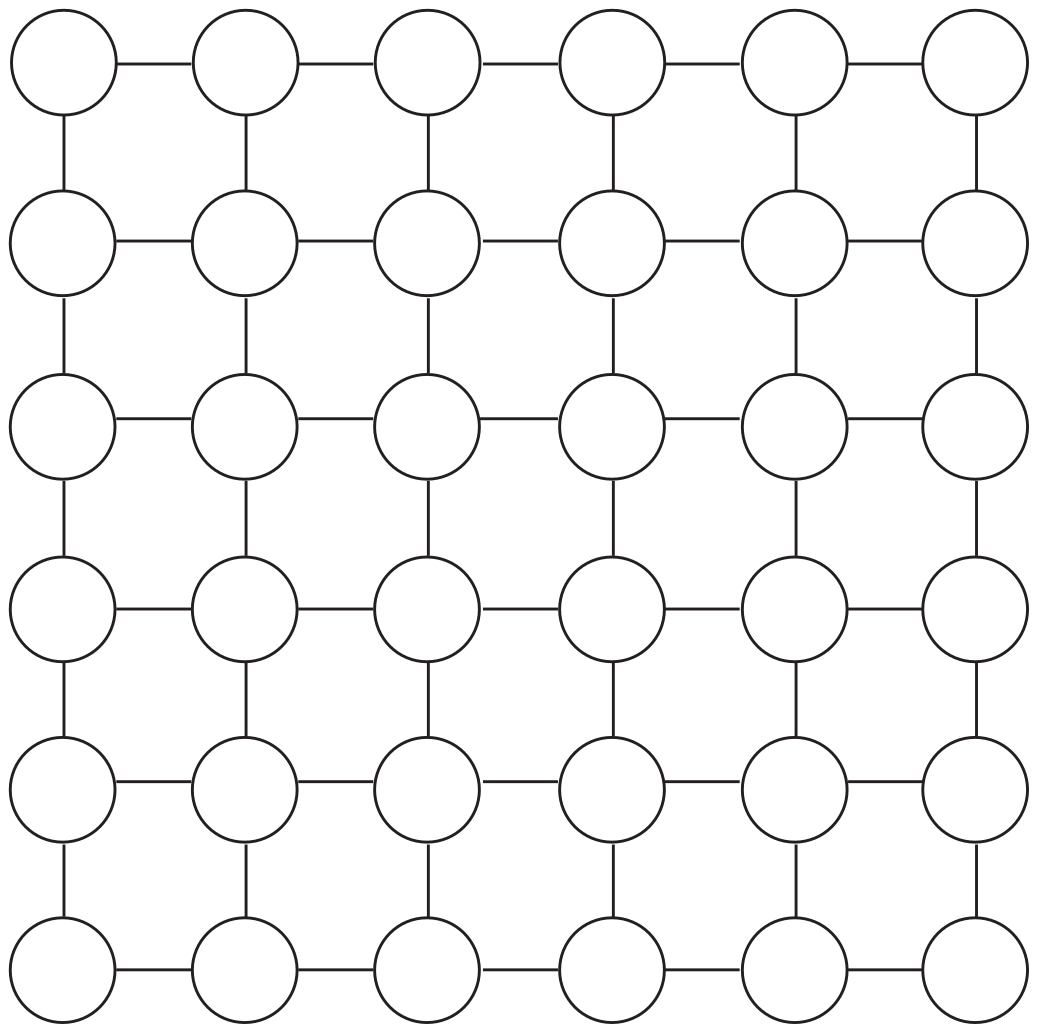
\includegraphics[width=0.4\linewidth]{media/p4.png}
\end{figure}

Each node $v$ in $G$ has a weight $w(v) > 0$.  You want to choose an independent set of nodes with maximum total weight.  That is, you want to choose a set of nodes $S$ with maximum total weight such that for any $v \in S$, none of $v$'s neighbors are in $S$.  To do this, consider the following greedy algorithm.  Let $V$ be the set of all nodes in $G$.  Choose the node in $V$ with the largest weight (breaking ties arbitrarily), add it to the independent set, then remove the node and all its neighbors from $V$.  Repeat this process until $V$ is empty.  Let $S$ be the output of this algorithm.   Solve the following problems.

\begin{enumerate}
\item Let $T$ be any independent set in $G$.  Show that for each node $v \in T$, either $v \in S$, or there is a neighbor $v'$ of $v$ with $v' \in S$ and $w(v) \leq w(v')$.
\item Show that the greedy algorithm is a 4-approximation.
\end{enumerate}

\solution{}
1. <1> If $v \in S$, then according to the definition of the independent set, we could get that for any neighbor    $v'$ of $v$, $v' \notin S$.

<2> If $v \notin S$, then according to the independent set, there exist at least one neighbor $v'$ of $v$ such that $v' \in S$. \\
And according to the greedy algorithm, we could get if for all neighbors $v'$ of $v$, $v'\in S$ has that $w(v')<w(v)$, the algorithm would choose $v$ before $v'$, which contradicts the greedy algorithm. So there must exist a neighbor $v'$ of $v$ such that $v' \in S$ and $w(v) \leq w(v')$.

So above all, we have proved that for each node $v \in T$, either $v \in S$, or there is a neighbor $v'$ of $v$ with $v' \in S$ and $w(v) \leq w(v')$.\\

2. Suppose that the greedy algorithm chooses the nodes consisting of $S$, and the optimal solution chooses the nodes consisting of $S^*$.\\

According to 1, we could get that for each node $v \in S$, either $v \in S^*$, or there is a neighbor $v'$ of $v$ with $v' \in S^*$ and $w(v) \leq w(v')$.\\

<1> If $v\in S$ and $v\in S^*$, then the weight of $v$ contributes the same in both $S$ and $S^*$.\\

<2> If $v\in S$ and $v\notin S^*$, then for the most extrame case, all the $4$ neighbors of $v$ are in $S^*$. According to the greedy's policy and analysis in 1, we could know that $w(v)>w(v')$, where $v'$ is any of the neighbors of $v$. So the most extrame case is that contribue $w(v)$ in $S$, and at most $4w(v')<4w(v)$ to $S^*$.\\

i.e. we could conclude that if $S^*$ removes a node $v$ from $S$, then for this modification, removing $v$ and adding its $4$ neighbors would increase the total weight of $S^*$ by at most $4w(v)$.\\

So we could get that the total weight of $S: w(S)$ is at least $\dfrac{1}{4}w(S^*)$, which is the total weight of $S^*$.\\
i.e.
$$w(S)\geq \dfrac{1}{4}w(S^*)$$

So above all, we have proved that the greedy algorithm is a 4-approximation.\\